\chapter{Interpretacja wyników}

W celu określenia jakości działania silnika kategoryzacyjnego przeprowadzono kilka testów. Testy polegały na przeprowadzeniu kategoryzacji obrazów pochodzących ze zbioru Caltech-101.\cite{CALTECH101}

Caltech-101 jest zbiorem obrazów przygotowanych na Kalifornijskim Uniwersytecie Technicznym (w skrócie \emph{Caltech}) przez Fei-Fei Li, Marca Andreetto oraz Marca Aurelio Ranzato. Zawiera obrazy nieobciążone ograniczeniami licencyjnymi podzielone na 101 kategorii.

Testy zostały przeprowadzone dla 2, 4 oraz 8 kategorii, dla zbiorów zawierających 1, 5, 10, 15, 20, 30 oraz 40 obrazów na kategorię. Poniżej znajdują się wykresy trafności dla poszczególnych przypadków. Liczbę klastrów ustalono na 1500. Kategorie testowe były następujące: samoloty, samochody, lampart, motocykle, budda, żyrandol, pianino.

\begin{figure}[h]
	\centering
	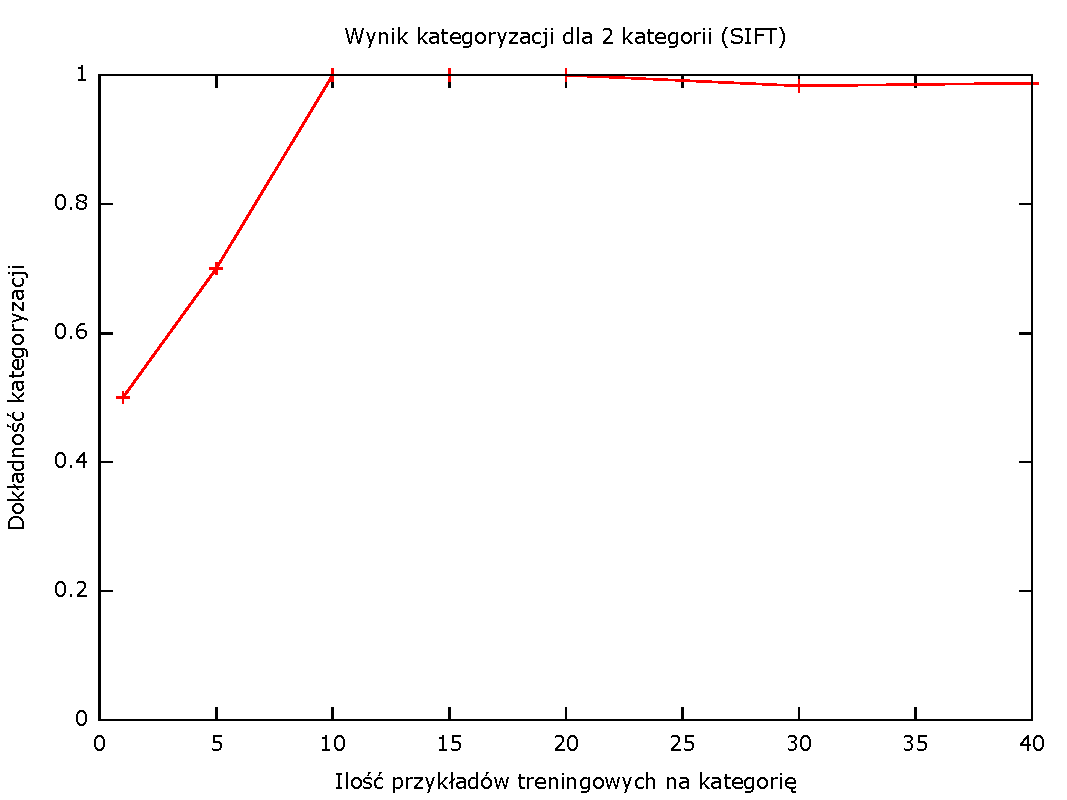
\includegraphics[scale=0.8]{graphics/04_interpretacja_wynikow/result-sift-2.pdf}
	\caption{ Wykres trafności dla uczenia 2 kategorii (SIFT), k=1500 }
	\label{fig:result-sift-2}
\end{figure}

\begin{figure}[h]
	\centering
	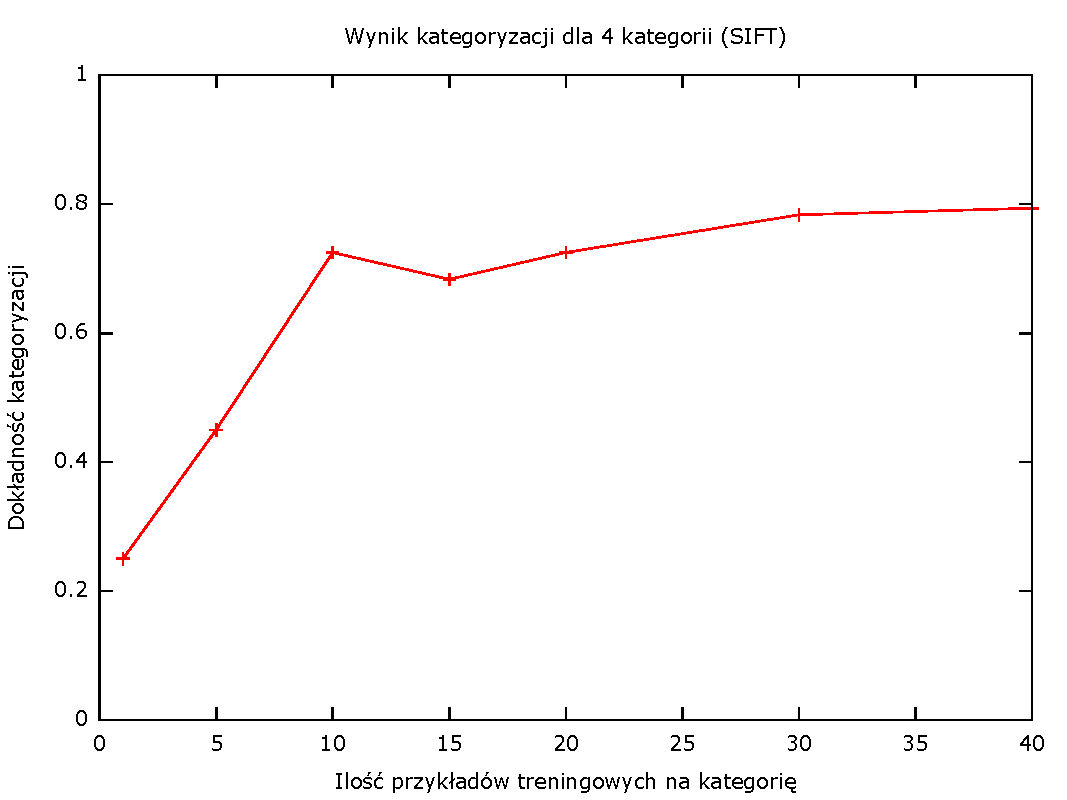
\includegraphics[scale=0.8]{graphics/04_interpretacja_wynikow/result-sift-4.pdf}
	\caption{ Wykres trafności dla uczenia 4 kategorii (SIFT), k=1500 }
	\label{fig:result-sift-4}
\end{figure}

\begin{figure}[h]
	\centering
	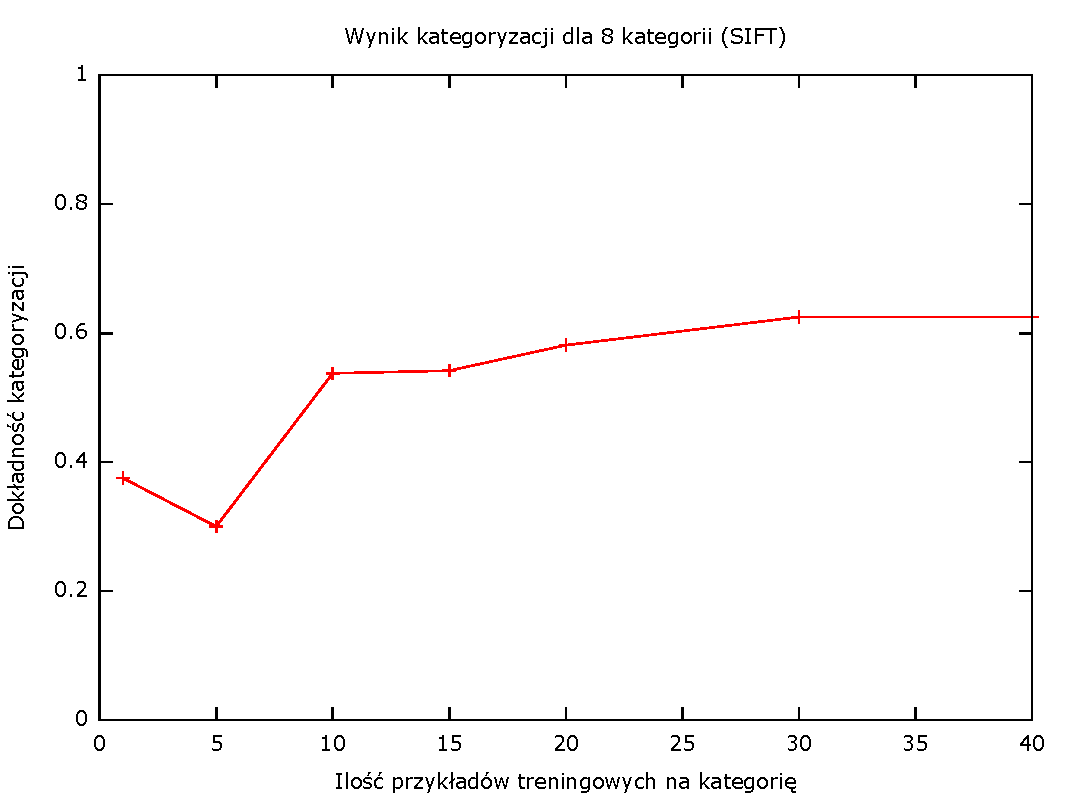
\includegraphics[scale=0.8]{graphics/04_interpretacja_wynikow/result-sift-8.pdf}
	\caption{ Wykres trafności dla uczenia 8 kategorii (SIFT), k=1500 }
	\label{fig:result-sift-8}
\end{figure}

\begin{figure}[h]
	\centering
	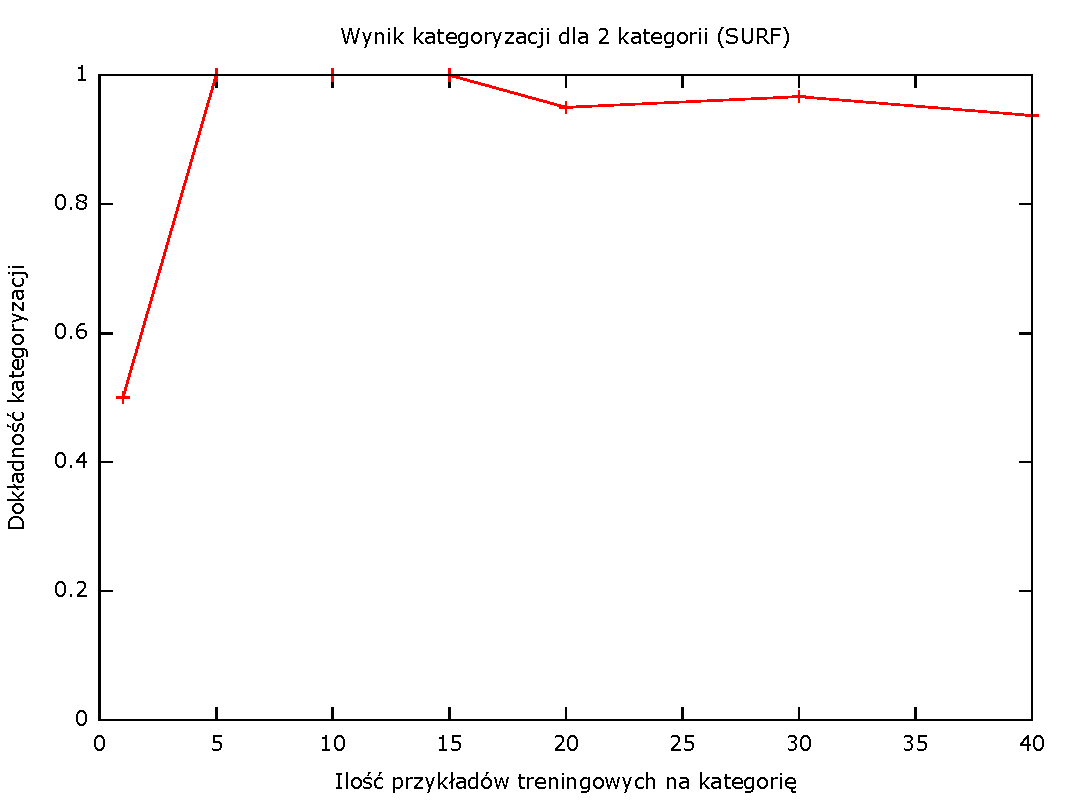
\includegraphics[scale=0.8]{graphics/04_interpretacja_wynikow/result-surf-2.pdf}
	\caption{ Wykres trafności dla uczenia 2 kategorii (SURF), k=1500 }
	\label{fig:result-surf-2}
\end{figure}

\begin{figure}[h]
	\centering
	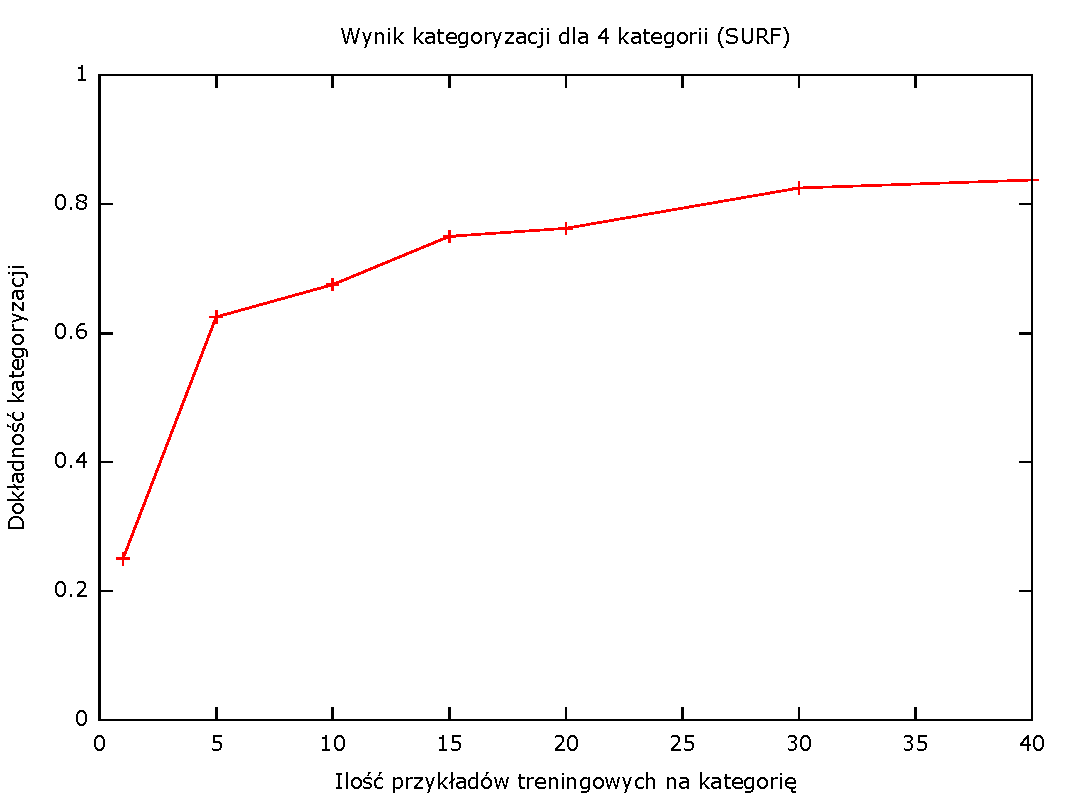
\includegraphics[scale=0.8]{graphics/04_interpretacja_wynikow/result-surf-4.pdf}
	\caption{ Wykres trafności dla uczenia 4 kategorii (SURF), k=1500 }
	\label{fig:result-surf-4}
\end{figure}

\begin{figure}[h]
	\centering
	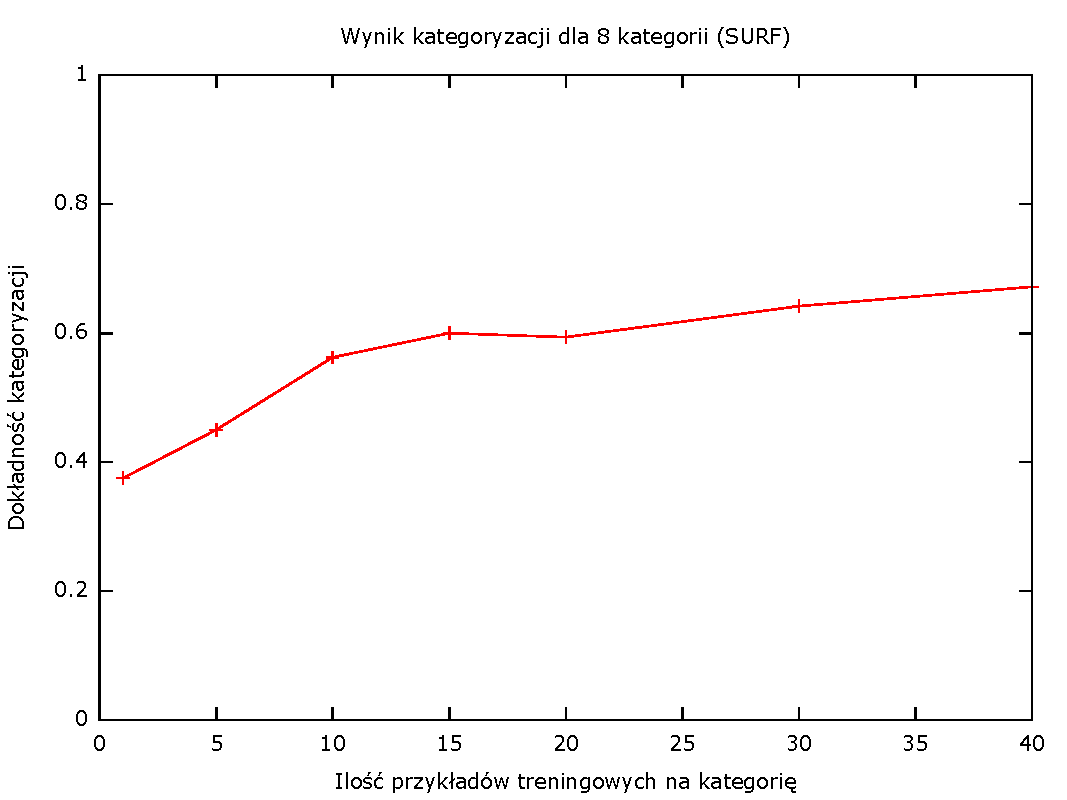
\includegraphics[scale=0.8]{graphics/04_interpretacja_wynikow/result-surf-8.pdf}
	\caption{ Wykres trafności dla uczenia 8 kategorii (SURF), k=1500 }
	\label{fig:result-surf-8}
\end{figure}

Wyniki dla algorytmów SURF i SIFT są zbliżone, jednakże dużo większa czasochłonność algorytmu SIFT jest zauważalna. Widać przewagę SIFT nad SURF w przypadku kategoryzacji dla 2 kategorii. Dokładności dla 2 oraz 4 kategorii są bardzo dobre: odpowiednio ok 90\% i ok. 80\% dla zbiorów uczących o czterdziestu elementach. Zauważalny jest spadek dokładności dla przypadku 8 kategorii, najlepszy wynik dla tego przypadku wyniósł 67.19\%. 

Dla przypadków 4 i 8 kategorii widoczny jest wzrost dokładności wraz ze wzrostem przykładów w zbiorze uczącym. Dla przypadku 2 kategorii doszło najprawdopodobniej do zjawiska zbytniego dopasowania klasyfikatora, ponieważ do pewnego momentu klasyfikator daje dobre rezultaty, a potem wraz ze wzrostem ilości przykładów, dokładność maleje.

Niezbyt dobre wyniki dla przypadku 8 kategorii mogły być związane z niewłaściwym doborem parametrów, dlatego postanowiono zmniejszyć liczbę klastrów do 500 i przeprowadzono ponowny test dla deskryptora SURF (rys. \ref{fig:result-surf-2-1500-500}, \ref{fig:result-surf-4-1500-500}, \ref{fig:result-surf-8-1500-500}).

\begin{figure}[h]
	\centering
	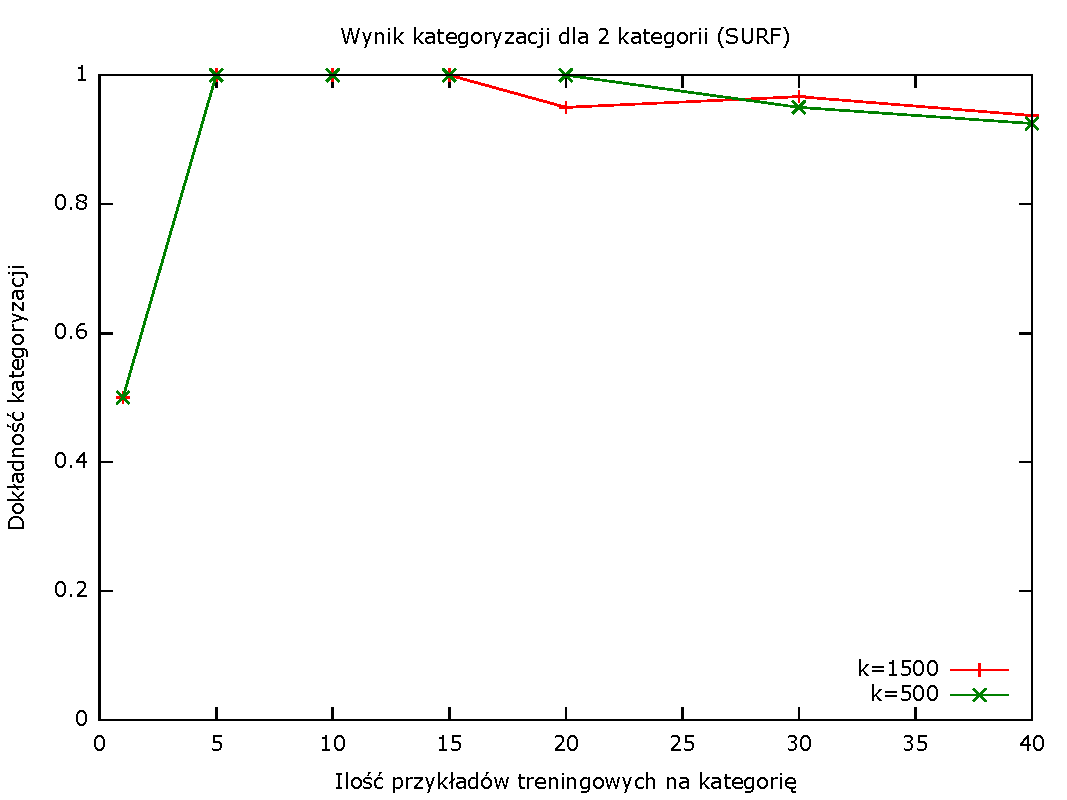
\includegraphics[scale=0.8]{graphics/04_interpretacja_wynikow/result-surf-2-1500-500.pdf}
	\caption{ Wykres trafności dla uczenia 2 kategorii (SURF), k=1500, k=500 }
	\label{fig:result-surf-2-1500-500}
\end{figure}

\begin{figure}[h]
	\centering
	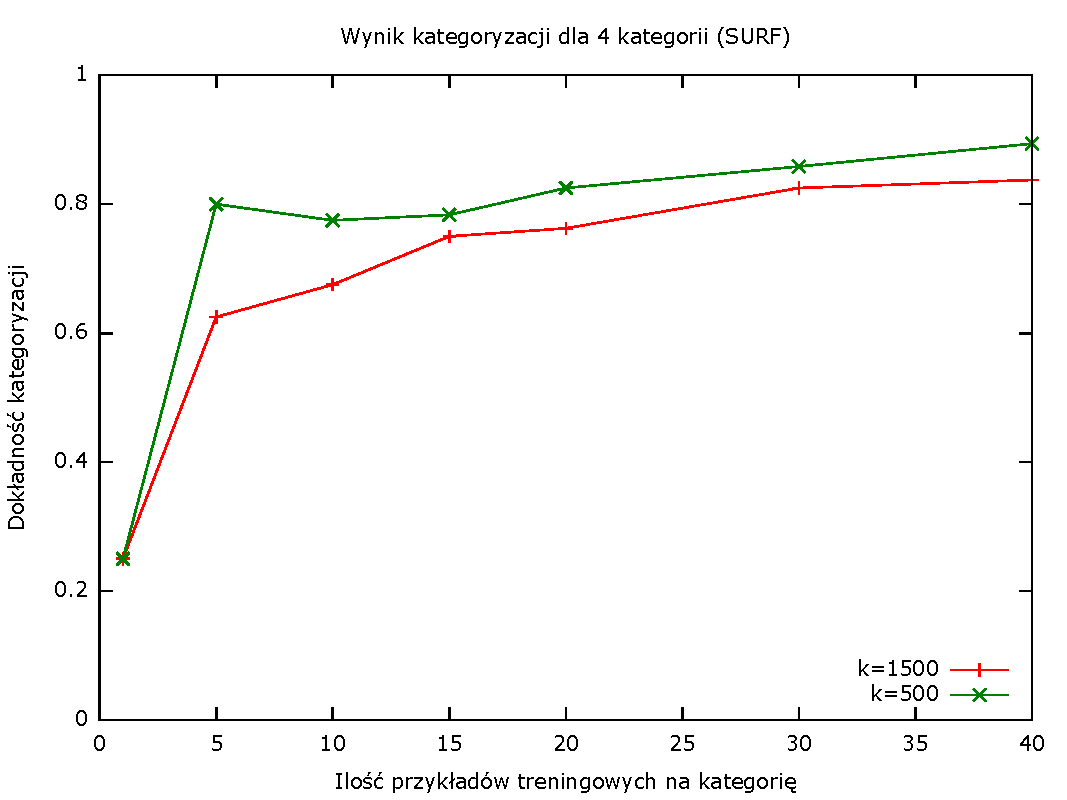
\includegraphics[scale=0.8]{graphics/04_interpretacja_wynikow/result-surf-4-1500-500.pdf}
	\caption{ Wykres trafności dla uczenia 4 kategorii (SURF), k=1500, k=500 }
	\label{fig:result-surf-4-1500-500}
\end{figure}

\begin{figure}[h]
	\centering
	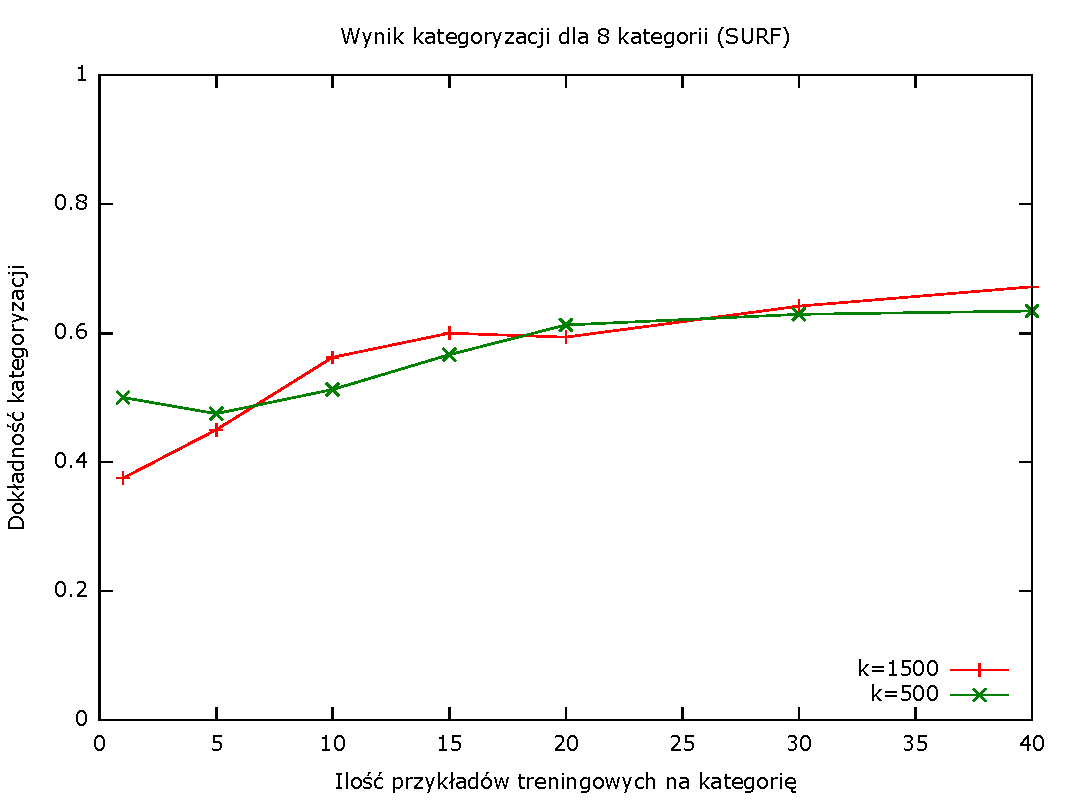
\includegraphics[scale=0.8]{graphics/04_interpretacja_wynikow/result-surf-8-1500-500.pdf}
	\caption{ Wykres trafności dla uczenia 8 kategorii (SURF), k=1500, k=500 }
	\label{fig:result-surf-8-1500-500}
\end{figure}

Zauważono znaczną poprawę dla przypadku 4 kategorii, niestety nie udało się poprawić wyniku dla 8 kategorii.